\documentclass[sigconf,nonacm]{acmart}
\settopmatter{printacmref=false}
\usepackage{subcaption}
\usepackage{booktabs}
\usepackage{float}
\usepackage{placeins}
\usepackage{pgfplots}
\usepackage{graphicx}
\usepackage{tikz}
\usetikzlibrary{positioning, shapes.geometric}
\renewcommand{\topfraction}{0.9}
\renewcommand{\bottomfraction}{0.8}
\setcounter{topnumber}{2}
\setcounter{bottomnumber}{2}
\setcounter{totalnumber}{4}
\setcounter{dbltopnumber}{2}
\renewcommand{\dbltopfraction}{0.9}
\renewcommand{\textfraction}{0.07}

%%
%% \BibTeX command to typeset BibTeX logo in the docs
\AtBeginDocument{%
  \providecommand\BibTeX{{%
    Bib\TeX}}}

%% Rights management information.  This information is sent to you
%% when you complete the rights form.  These commands have SAMPLE
%% values in them; it is your responsibility as an author to replace
%% the commands and values with those provided to you when you
%% complete the rights form.
\setcopyright{none}
\copyrightyear{2025}
\acmYear{2025}
\acmDOI{}

%% These commands are for a PROCEEDINGS abstract or paper.
\acmConference[15-689]{Independent Study}{Spring 2025}{Carnegie Mellon University}

\acmISBN{}


\begin{document}

\title{How Good is Good Cardinality Estimation?}

\author{Aarrya Saraf supervised by Dr. Armaghan "Rumi" Naik}
\affiliation{%
  \institution{Carnegie Mellon University}
  \city{Pittsburgh}
  \state{PA}
  \country{USA}
}


\renewcommand{\shortauthors}{Saraf and Naik}

\begin{abstract}
Relational Database Management Systems make use of cardinality estimates for every part of a query plan during query optimization to be able to select the best estimated option. It is long known that cardinality estimates are poor and recent work has included feedback loops and machine learning to help make them "good" or robustness and adaptivity making them almost agnostic to bad estimates. In this paper, we review the current state of the field, give a mathematical model of query optimization's dependence on cardinalities, and answer how "good" cardinalities really need to be to have a good plan. 
\end{abstract}

%%
%% The code below is generated by the tool at http://dl.acm.org/ccs.cfm.
%% Please copy and paste the code instead of the example below.
%%
\begin{CCSXML}
<ccs2012>
<concept>
<concept_id>10002951.10002952.10003190.10003192</concept_id>
<concept_desc>Information systems~Database query processing</concept_desc>
<concept_significance>500</concept_significance>
</concept>
<concept>
<concept_id>10002951.10002952.10003190.10003192.10003203</concept_id>
<concept_desc>Information systems~Query optimization</concept_desc>
<concept_significance>500</concept_significance>
</concept>
<concept>
<concept_id>10003752.10003809.10010172</concept_id>
<concept_desc>Theory of computation~Database query processing and optimization (theory)</concept_desc>
<concept_significance>300</concept_significance>
</concept>
</ccs2012>
\end{CCSXML}

\ccsdesc[500]{Information systems~Database query processing}
\ccsdesc[500]{Information systems~Query optimization}
\ccsdesc[300]{Theory of computation~Database query processing and optimization (theory)}

\keywords{DuckDB, Cardinality Estimation, Query Optimization}

\maketitle

\section{Introduction}

It is widely believed that suboptimal query plans are often selected due to inaccurate cardinality estimation. However notice that as long as the right physical plan is chosen in the end, potentially a great deal of imprecision in the cardinality estimates may be immaterial. So a more careful analysis would distinguish between the precision of a cardinality estimate and its accuracy. In this light it is to our knowledge not yet known whether optimizers are “right for the wrong reasons” enough of the time that would limit the potential improvement from a more accurate cardinality estimator.

This has two major implications. First, we seek to characterize how often oracle-quality join cardinalities would give rise to a different physical plan selection than the DuckDB baseline estimator would. Secondly, we are interested in understanding what bias / variance tradeoff is necessitated by a potential statistical estimator of cardinality in order to materially improve on the presumably low bias, high variance existing estimator in DuckDB.

We will start by giving a mathematical model of query optimization and then ultimately present a topology of choice architecture for DuckDB on TPCDS Showing <TBD>

\section{Related Work}

The critical role of cardinality estimation in query optimization has been heavily scrutinized over the last decade. A foundational contribution to this discussion is the work by Leis et al. in "How Good Are Query Optimizers, Really?". They demonstrated that traditional cardinality estimates degrade exponentially as the number of joins increases, often causing optimizers to select disastrously slow physical plans.

To understand the true impact of these estimation errors, researchers have increasingly relied on exact-cardinality baselining. The most critical benchmark in this space is the recent work by Lee, Dutt, et al. (2023), who developed a custom cardinality injection API for Microsoft SQL Server. By bypassing the engine’s built-in cost model and injecting exact, true cardinalities for every logical sub-expression, they systematically quantified how often the optimizer is "right for the wrong reasons." Their evaluation revealed that execution-time techniques heavily mask estimation errors. Our work directly adapts this methodology—building a robust, iterative injection API to feed exact cardinalities into the query optimizer—but applies it to the highly vectorized, analytical architecture of DuckDB. This builds on foundational optimizer testing frameworks (Chaudhuri et al., 2009) that use perfect cardinalities to isolate whether sub-optimal performance stems from bad estimates or a flawed search strategy.

Recent research has also applied exact cardinality injection to resolve estimation errors for single-table vector similarity predicates, such as the Exqutor system (Kim et al., 2026). However, while Exqutor focuses on estimating the selectivity of high-dimensional vector filters prior to execution, our focus remains squarely on the exponential estimation errors generated by multi-way relational joins and their impact on physical plan choice.

Understanding how accurate these join estimates actually need to be requires mapping out the optimizer's "plan space." Foundational work on Plan Diagrams (Reddy & Haritsa, 2005) demonstrated that the space of optimal plans is highly complex but can often be reduced to a much smaller subset of robust choices without major performance regressions. Building on this simplified plan space, research on coresets has shown that a tiny subset of plans can serve as robust candidates for an entire query template space.

Our work synthesizes these concepts to establish a definitive ground truth. While execution-time features like DuckDB's Robust Plan Trees (RPT) mask estimation errors mid-flight, often countering the exact failures identified by Leis et al., we aim to reveal the true performance ceiling of the optimizer itself. By iteratively injecting exact, oracle-quality join cardinalities into DuckDB, we baseline the engine's inherent scope for improvement. This mapping of the "topology of choice architecture" quantifies exactly how often the DuckDB optimizer is saved by its execution engine versus making genuinely optimal planning decisions. While we demonstrate these structural boundaries using TPC-DS, our injection framework and findings generalize to any relational benchmark.

\section{Mathematical Model of Query Optimization}
Let us fix a query $Q$. Every query corresponds to an equivalence class of Logical Plans $\mathbf{L'}_Q$ which in turns corresponds to an equivalence class of Physical Plans $\mathbf{P'}_Q$. Foe example a query can talk about joining two trees, a logical plan would show that join, a physical plan would flesh it out as a hash join or sort-merge join (after a sort). These plans are represented as trees. The leaves are the tables, the nodes have one (such as a sort) or two children (such as a join). To accommodate joins between multiple tables, optimizers typically chain them. We note that not every plan in $L'_Q$ or $P'_Q$ has the same number of nodes, for example nested queries. We represent by $L_Q$ all the logical plans in $L'_Q$ that have the minimum number of nodes $k$. These trees also maintain "interesting" characteristics for the data. These are properties of the data such as sorting. 
If an oracle existed for query optimization we could imagine it would be able to run every physical plan in $P_Q$ and select the best one. Given this, we define 

Hence, if $LO$ is the set of logical operators
$IC$ is the set of interesting characteristics (e.g. sorting or partitioning)
$CE$ is the set of cardinality estimate which is the same as $\mathbb{R^+}$, then our logical plan tree

\begin{equation}
\begin{aligned}
T_Q = \{ \\
    &(lo, ic, ce, l, r) \\
    \mid \, &lo \in LO \\
    &ic \in IC\\
    &ce \in CE\\
    &l, r \in T \cup \{\bot\} \\
    \}
\end{aligned}
\end{equation}

$l$ and $r$ represent the right and left children which may or may not exist (leaves are equipped with the project operator). Then by using some sort of ordering on the tree (such as infix), we arrive at the following representation 

\begin{equation}
\begin{aligned}
T_Q = \{ \\
    &(lo, ic, ce)^k \\
    \mid \, &lo \in LO \\
    &ic \in IC\\
    &ce \in CE\\
    \}
\end{aligned}
\end{equation}

\subsection{What "Best" Plan Really Means}

Defining a "best" plan can be tricky. Due to factors such as the cache, there is variance of the same plan being run multiple times. Due to robustness and adaptive techniques, some "bad" plans can be consistently executed with extremely little variance at very fast speeds. We use the following metric. In a cold cache, we run each plan five times, and pick the fastest run. Whichever plan gives the fastest run is the "best". 

\subsection{Cost Estimation in Moderns DBMSs}

Modern DBMSs approximate this cost in multiple ways. Those like DuckDB try and measure the amount of data flowing through each node of the plan. For those like Postgres, they use weights that you must determine by running some calculations. Recent times have seen Machine Learning methods which try and skip the cost approach to directly spit out a plan. These did not see much success, instead there are also machine learning methods which try and assign costs to such trees. All but the third one rely on cardinality estimates at each node. Some DBMSs here use simple techniques and statistics like equihistograms to store table data cheaply and use the independence assumption to estimate joins. This is a good approximation of storing the marginal distribution. Simply storing the joint distribution is not possible as it might be far larger than the size of the data itself. Hence, we see large issues when estimating the joint distribution. Consider the following queries:
\begin{verbatim}
    SELECT *
    FROM Brands B
    JOIN Models M ON B.brand_id = M.brand_id
    WHERE B.name = 'Honda' AND M.name = 'Camry';
\end{verbatim}

and 

\begin{verbatim}
    SELECT *
    FROM Brands B
    JOIN Models M ON B.brand_id = M.brand_id
    WHERE B.name = 'Honda' AND M.name = 'Civic';
\end{verbatim}

The former will result in a zero result while the latter will be a full join. The cardinality estimate in these areas, however, will be $P(Honda)\times P(Camry)$ and $P(Honda)\times P(Civic)$ which are way off. Because of the importance of cardinality estimation in cost estimation, this often leads to bad plans. 

Mathematically speaking, the oracle has an oracle cost function
$$ \hat{cost}_Q: P_Q\to \mathbb{R^+}$$

that we try to approximate as follows:
$$ {cost}_Q: T_Q\to (\mathbb{R^+}, P_Q)$$

In essence, for some logical plans, we get the cheapest corresponding physical plan. Then we for all the explored logical plans, we select the cheapest physical plan. 

\subsection{Properties of The Cost Functions}

For our fixed query, we will now try and answer how things change based on the changes in the estimates of the cardinalities of the joins of the underlying data. We can imagine this as the properties of a function from the space of estimates of join cardinalities to the cost of the corresponding physical plan. 

\begin{enumerate}
    \item The cost function is locally constant over any axis of the cardinality estimate everywhere except a finite negligible set measure theoretically. This describes a step function in multiple dimensions. 
    \item There are only finitely many plans which the optimizer will consider. This means that even as the estimates grow worse and worse, our plan does not get worse after a point (the execution of the same plan might be worse due to bad memory allocation but that is not the same as the plan getting worse). 
    \item For a fixed optimizer, there exists at least one subspace of plans that is the best the optimizer can do. We would like to profile to see how much effort and information it takes us to get there, and how wide our margin of error really is. 
    \item Quite importantly, there is no need for there to be one subspace that maps to the optimum plan. If multiple subspaces map to the optimal plan they do not need to be connected either. 
    \item Similarly, there might be multiple optimal plans. This means that we can have potentially multiple unconnected subspaces. 
    \item Our graph also might contain local extrema that we must be aware of. 
\end{enumerate}

\begin{figure*}[t] % Use figure* to span both columns at the top
    \centering
    
    % --- Subfigure (A): Point Discontinuity (Original) ---
    \begin{subfigure}[b]{0.3\textwidth}
        \centering
        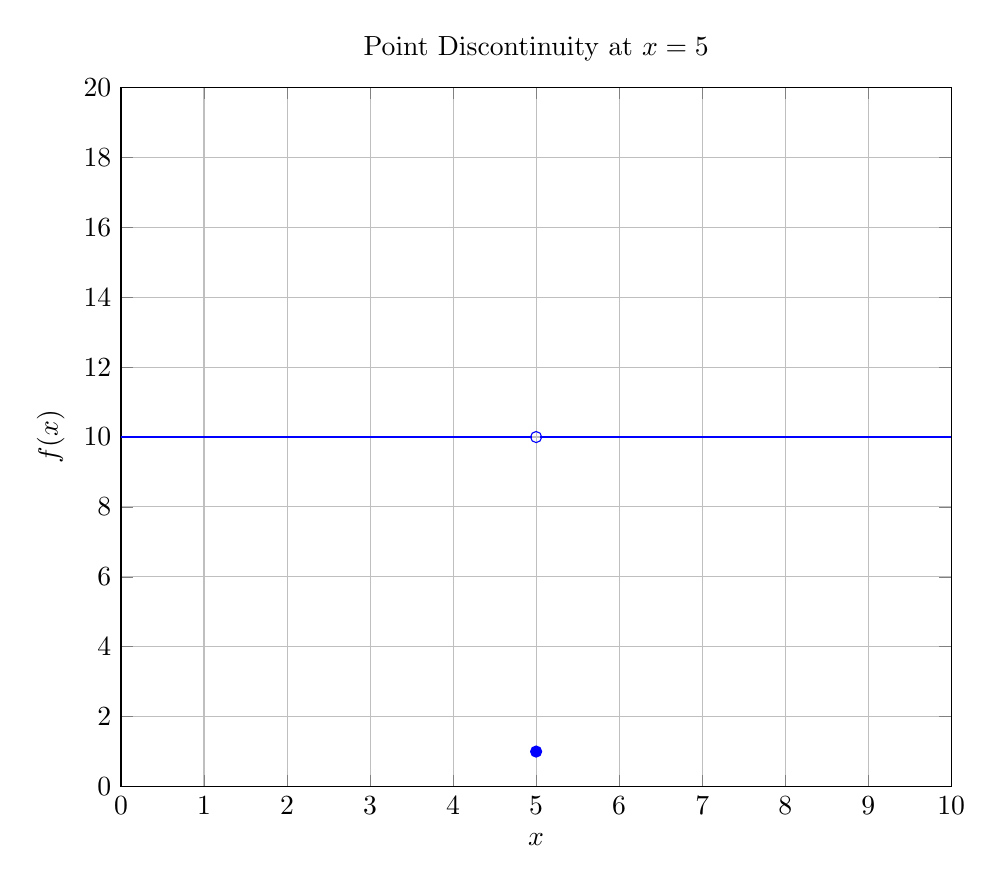
\begin{tikzpicture}
            \begin{axis}[
                width=\textwidth,
                xmin=0, xmax=10,
                ymin=0, ymax=20,
                xlabel={$x$},
                ylabel={$f(x)$},
                grid=major,
                title={Point Discontinuity at $x=5$}
            ]
                % Constant lines with small gaps
                \addplot[blue, thick, domain=0:4.95] {10};
                \addplot[blue, thick, domain=5.05:10] {10};
                
                % Points: [5]=1 (Closed), but excluded from y=10 line (Open)
                \addplot[blue, mark=*, only marks] coordinates {(5,1)};
                \addplot[blue, fill=white, mark=o, only marks] coordinates {(5,10)};
            \end{axis}
        \end{tikzpicture}
        \caption{$f(x)=1$ at $x=5$, else $10$.}
    \end{subfigure}
    \hfill
    % --- Subfigure (B): Simple Step (Refined original) ---
    \begin{subfigure}[b]{0.3\textwidth}
        \centering
        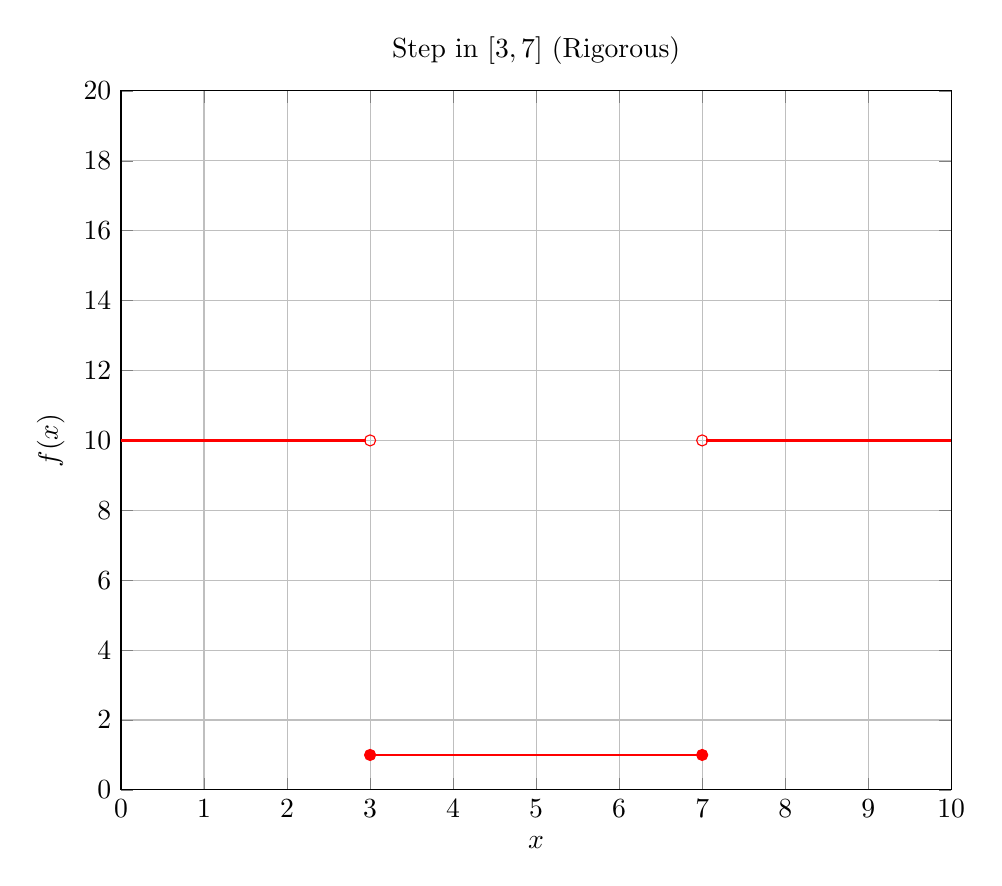
\begin{tikzpicture}
            \begin{axis}[
                width=\textwidth,
                xmin=0, xmax=10,
                ymin=0, ymax=20,
                xlabel={$x$},
                ylabel={$f(x)$},
                grid=major,
                title={Step in $[3,7]$ (Rigorous)}
            ]
                % Constant lines with small gaps
                \addplot[red, thick, domain=0:2.95] {10};
                \addplot[red, thick, domain=3.05:6.95] {1};
                \addplot[red, thick, domain=7.05:10] {10};
                
                % Markers: Boundaries [3,7] included at y=1 (Closed), but holes at y=10 (Open)
                \addplot[red, mark=*, only marks] coordinates {(3,1) (7,1)};
                \addplot[red, fill=white, mark=o, only marks] coordinates {(3,10) (7,10)};
            \end{axis}
        \end{tikzpicture}
        \caption{$f(x)=1$ for $x \in [3,7]$, else $10$.}
    \end{subfigure}
    \hfill
    % --- Subfigure (C): The New Mixed Function ---
    \begin{subfigure}[b]{0.3\textwidth}
        \centering
        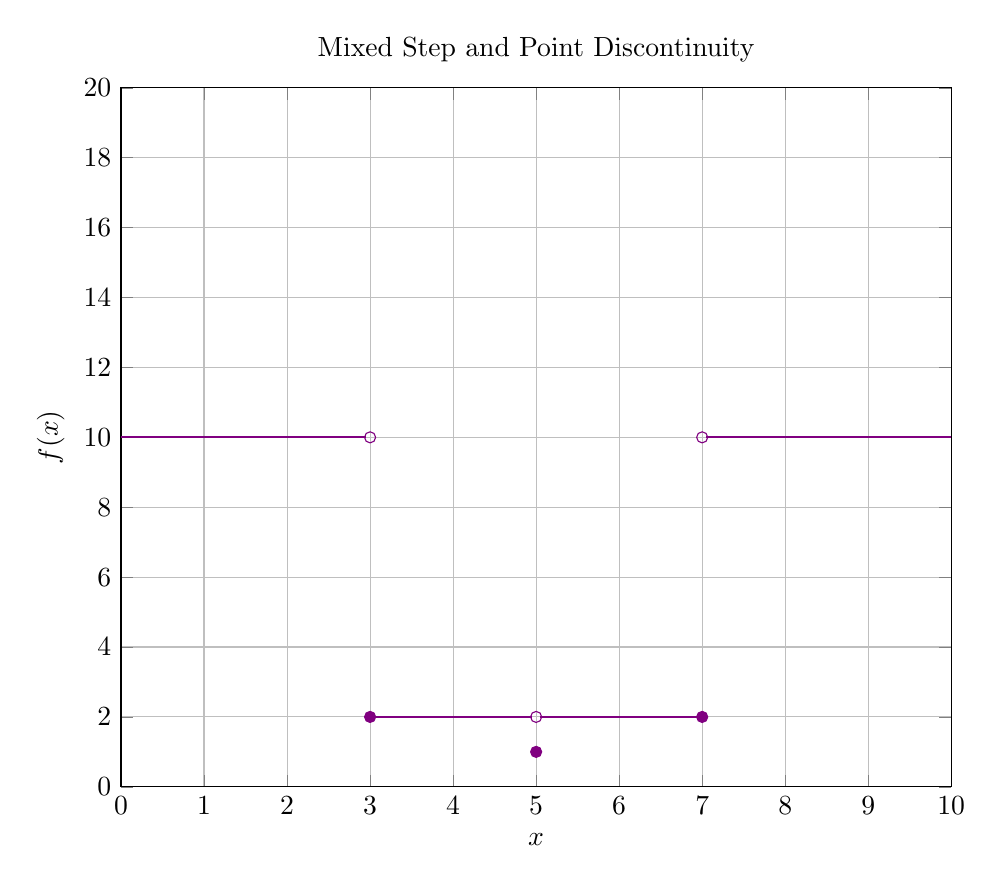
\begin{tikzpicture}
            \begin{axis}[
                width=\textwidth,
                xmin=0, xmax=10,
                ymin=0, ymax=20,
                xlabel={$x$},
                ylabel={$f(x)$},
                grid=major,
                title={Mixed Step and Point Discontinuity}
            ]
                % 1. Horizontal segments (no vertical lines, including the hole at x=5)
                \addplot[violet, thick, domain=0:2.95] {10};
                \addplot[violet, thick, domain=3.05:4.95] {2};
                \addplot[violet, thick, domain=5.05:6.95] {2};
                \addplot[violet, thick, domain=7.05:10] {10};
                
                % 2. Closed circles: The points where f is defined exactly.
                % Defined at: 3 (level 2), 7 (level 2), and 5 (level 1).
                \addplot[violet, mark=*, only marks] 
                    coordinates {(3,2) (7,2) (5,1)};
                
                % 3. Open circles: The "holes" (excluded boundaries).
                % Holes at: Boundaries of [0,3) and (7,10] (at y=10) and boundary of (3,5) U (5,7] (at y=2).
                \addplot[violet, fill=white, mark=o, only marks] 
                    coordinates {(3,10) (7,10) (5,2)};
            \end{axis}
        \end{tikzpicture}
        \caption{$f(5)=1$, $x \in [3,7]\setminus\{5\}$ is $2$, else $10$.}
    \end{subfigure}

    \caption{Bla bla bla}
    \label{fig:step-functions}
\end{figure*}

% --- Conceptual Diagram of Subspaces ---
% Requires \usepackage{tikz} in your preamble.

\begin{figure}[H]
    \centering
    % Using \linewidth is safer for column constraints in sigconf
    \resizebox{\linewidth}{!}{
        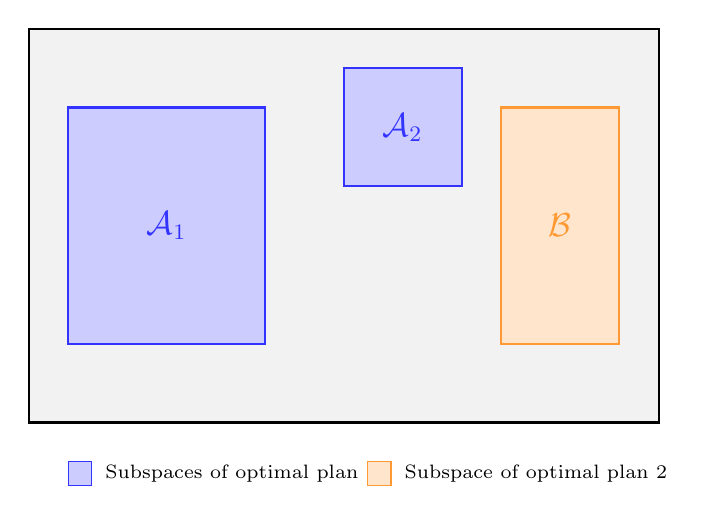
\begin{tikzpicture}[x=1cm, y=1cm] % Explicitly set unit vectors
            % 1. Background Domain
            \draw[thick, fill=gray!10] (0,0) rectangle (8,5);

            % 2. Subspaces for Property 1 (Blue)
            \draw[fill=blue!20, draw=blue!80, thick] (0.5, 1.0) rectangle (3.0, 4.0);
            \draw[fill=blue!20, draw=blue!80, thick] (4.0, 3.0) rectangle (5.5, 4.5);
            \node[blue!80, font=\large] at (1.75, 2.5) {$\mathcal{A}_1$};
            \node[blue!80, font=\large] at (4.75, 3.75) {$\mathcal{A}_2$};
            
            % 3. Subspace for Property 2 (Orange)
            \draw[fill=orange!20, draw=orange!80, thick] (6.0, 1) rectangle (7.5, 4);
            \node[orange!80, font=\large] at (6.75, 2.5) {$\mathcal{B}$};

            % 4. Legend (Using a node for easier positioning)
            \begin{scope}[shift={(0.5, -0.8)}] % Changed y from 0.3 to -0.8
                \draw[fill=blue!20, draw=blue!80] (0,0) rectangle (0.3,0.3);
                \node[right, font=\scriptsize] at (0.35, 0.15) {Subspaces of optimal plan 1};
                
                \draw[fill=orange!20, draw=orange!80] (3.8,0) rectangle (4.1,0.3); % Adjusted x for spacing
                \node[right, font=\scriptsize] at (4.15, 0.15) {Subspace of optimal plan 2};
            \end{scope}
        \end{tikzpicture}
    }
    \caption{space of cardinalities mapping to plans visualized}
    \label{fig:subspaces}
\end{figure}

\section{Methodology}
\label{sec:methodology}

We study cardinality estimation in a custom fork of DuckDB by modifying the join-order cardinality estimator and by driving repeatable Python benchmarks over TPC-DS. The core idea is unchanged: intervene at logical join cardinality estimation, log enough context to reconstruct keys and optional \texttt{COUNT(*)} queries, optionally overwrite estimates from \texttt{actual\_cardinality.json}, and compare physical plans to vanilla. What follows reflects the \emph{current} harness (unified driver, stricter injectability rules, and richer verification), not the earliest prototype.

\subsection{DuckDB Instrumentation}

The modified cardinality estimator logs one block per logical join considered during optimization. Each block includes the relation set, relation bindings, filter predicates, per-relation input cardinalities, parent-split context, edge signature, occurrence index (\texttt{CtxOcc}) to disambiguate repeated contexts, and either an estimated cardinality or an injected value. An \texttt{ESTIMATION\_DETAIL} line records numerator, denominator, raw model output, and related factors so the native formula is visible even when a later line shows an injected cardinality.

Injection is keyed by the full logical-join string (optionally prefixed when \texttt{DUCKDB\_FEEDBACK\_PLAN\_FINGERPRINT} namespaces keys for feedback experiments). Values are read from \texttt{actual\_cardinality.json} (path overridable via \texttt{DUCKDB\_ACTUAL\_CARDINALITY\_JSON}). The estimator also emits \texttt{SQL\_COUNT\_QUERY}, \texttt{SQL\_COUNT\_REASON}, coverage metadata, and---when the fork is built with the corresponding shell support---\texttt{SQL\_COUNT\_INJECTABLE} / \texttt{SQL\_COUNT\_INJECTABLE\_REASON} so the Python side can skip oracle keys that are not safe to treat as standalone \texttt{COUNT(*)} closures. Auxiliary \texttt{EDGE\_COUNT\_QUERY} and \texttt{BASE\_CARD\_QUERY} lines support diagnosis; not every join yields executable SQL.

\subsection{Workload and Execution Harness}

Queries come from DuckDB's \texttt{tpcds\_queries()} for selected query ids. Each phase invokes the DuckDB CLI as a subprocess with a fixed database path, writing the cardinality log and profiling output under the repository root unless overridden by environment variables (\texttt{DUCKDB\_CARDINALITY\_LOG}, \texttt{DUCKDB\_ACTUAL\_CARDINALITY\_JSON}, \texttt{DUCKDB\_...}).

\textbf{Vanilla.} Run the query once with JSON profiling (\texttt{PRAGMA enable\_profiling}, detailed mode) to obtain the executed physical plan and a SHA-based \emph{plan fingerprint} derived from a canonical structural text (operators, join conditions, filters, tables, projections, etc., excluding volatile runtime fields).

\textbf{Feedback loop.} Start from an empty injection file. Each iteration: clear the log, profile the query, parse joins from the profile and logical lines from the log, match safe pairs, and append or update \texttt{actual\_cardinality.json}. Stop on structural convergence (two consecutive identical plan texts), oscillation (a plan text repeats), or an iteration cap. The harness can use a separate \texttt{duckdb\_feedback} binary (legacy join-order build) when present; otherwise it falls back to the main binary. The final run reports iterations, distinct plan count, convergence flags, and the number of cardinality-log lines marked \texttt{INJECTED} on the last completed iteration.

\textbf{Oracle injection.} Run \texttt{EXPLAIN} (no execution) to populate the cardinality log, then---subject to injectability and ambiguity rules---execute each accepted \texttt{SQL\_COUNT\_QUERY} (or skip / synthesize only when explicitly allowed) to build an oracle map, write it to JSON, and profile the full query with injection active. By default the oracle phase \emph{reuses} the vanilla JSON profile from the unified driver (\texttt{skip\_baseline\_phase}) so baseline work is not duplicated. Default strict mode skips oracle keys when the same \texttt{RelSets} tuple appears with multiple distinct \texttt{SQL\_COUNT\_QUERY} texts in one explain pass (\texttt{--oracle-permissive-context} relaxes this).

\subsection{Unified benchmark driver}

\texttt{unified\_benchmark.py} runs vanilla $\rightarrow$ feedback $\rightarrow$ oracle for each query with a single shared configuration (database path, log paths, binaries). It writes \texttt{unified\_benchmark\_results.csv} and \texttt{unified\_benchmark\_summary.txt}, and can mirror oracle-style diagnostics to \texttt{unified\_results.log}. The CSV is intentionally compact: it records \texttt{plan\_relation} (five-way classification of fingerprint equality among vanilla, feedback, and oracle), sparse boolean columns (errors and ``vanilla failed'' only when true), iteration metadata, \texttt{n\_inj\_feedback} / \texttt{n\_inj\_oracle} (counts of log lines marked injected on the last feedback iteration and on the oracle run), \texttt{n\_oracle\_keys} (size of the oracle map written to JSON), a flag when feedback's injected-line count exceeds the oracle phase's count \emph{and} the oracle map was non-empty (a diagnostic for asymmetric injection intensity), and oracle alarm counts. Full fingerprints remain in the text summary for debugging, not in the CSV.

\subsection{Verification and validity checks}

\textbf{Feedback.} From the second iteration onward, verify prior JSON against the log, check injected markers, and compare injected values to executed cardinalities for matched joins, with explicit handling for plan changes and CTE keys.

\textbf{Oracle.} Verify injected cardinalities agree with the oracle map (V1-style), coverage of oracle keys in the log, keys that were not injected when the plan diverges (informational), CTE injection warnings, and strict RelSets-SQL skip reporting. \textbf{V6 (on by default):} on the injected run's JSON profile, compare estimated vs.\ executed cardinalities for physical join operators that align with injected multi-table logical joins (symmetric relative error threshold; disambiguation when the same table multiset appears on multiple injected lines). Optional modes widen V6 to all operators or disable it for legacy comparisons.

When the oracle plan fingerprint differs from vanilla, the harness optionally runs five timed executions of each plan to surface wall-clock regressions or improvements; this is orthogonal to V6's cardinality agreement check.

\subsection{Caveats}

String keys remain sensitive to optimizer context and evaluation order. ``Oracle'' means exact cardinalities only where the logged counting query (or permitted synthesis) matches the join slot's relational semantics; partial maps remain possible by construction. Structural convergence in feedback does not imply all intermediate cardinalities have been corrected. Plan fingerprints are coarse summaries of physical structure. Comparing \texttt{n\_inj\_feedback} to \texttt{n\_inj\_oracle} counts log-line injections, not necessarily the same multiset of logical joins across phases. The unified driver enforces consistent DB and binaries across phases, but empirical tables in this revision are omitted until the harness is rerun for publication.

\section{Conclusion}

\bibliographystyle{ACM-Reference-Format}
\bibliography{references}

\appendix
\input{appendix}

\end{document}
